%%%%%%%%%%%%%%%%%%%%%%%%%%%%%%%%%%%%
% This is the template for submission to MICRO 2017
% The cls file is modified from 'sig-alternate.cls'
%%%%%%%%%%%%%%%%%%%%%%%%%%%%%%%%%%%%

\documentclass{sig-alternate}
\usepackage{mathptmx} % This is Times font

\usepackage{fancyhdr}
\usepackage[normalem]{ulem}
\usepackage[hyphens]{url}
\usepackage[sort,nocompress]{cite}
\usepackage[final]{microtype}
\usepackage{flushend}
% Always include hyperref last
\usepackage[bookmarks=true,breaklinks=true,letterpaper=true,colorlinks,linkcolor=black,citecolor=blue,urlcolor=black]{hyperref}

% Ensure letter paper
\pdfpagewidth=8.5in
\pdfpageheight=11in

%%%%%%%%%%%---SETME-----%%%%%%%%%%%%%
\newcommand{\microsubmissionnumber}{XXX}
%%%%%%%%%%%%%%%%%%%%%%%%%%%%%%%%%%%%

\fancypagestyle{firstpage}{
  \fancyhf{}
  \renewcommand{\headrulewidth}{0pt}
  \fancyhead[C]{\vspace{15pt}\normalsize{MICRO 2017 Submission
      \textbf{\#\microsubmissionnumber} -- Confidential Draft -- Do NOT Distribute!!}} 
  \fancyfoot[C]{\thepage}
}

\pagenumbering{arabic}

%%%%%%%%%%%---SETME-----%%%%%%%%%%%%%
\title{Guidelines for Submission to MICRO 2017} 
%%%%%%%%%%%%%%%%%%%%%%%%%%%%%%%%%%%%

\begin{document}
\maketitle
\thispagestyle{firstpage}
\pagestyle{plain}



%%%%%% -- PAPER CONTENT STARTS-- %%%%%%%%

\begin{abstract}
Heterogeneous computing with GPUs integrated on the same chip as CPUs is ubiquitous,
and to increase programmability many of these systems support virtual address accesses
from GPU hardware.
\end{abstract}

\section{Introduction}

%This document provides instructions for submitting papers to the 50th
%International Symposium on microarchitecture (MICRO), 2017.  In an
%effort to respect the efforts of reviewers and in the interest of
%fairness to all prospective authors, we request that all submissions
%to MICRO 2017 follow the formatting and submission rules detailed
%below. Submissions that violate these instructions may not be reviewed,
%at the discretion of the program chairs, in order to maintain a review
%process that is fair to all potential authors.
%
%
%This document is itself formatted using the MICRO-50 submission format.
%The content of this document mirrors that of the submission
%instructions that appear on
%\href{http://www.microarch.org/micro50/Submission/}{this website}.
%
%All questions regarding paper formatting and submission should be directed
%to the program chairs.

\subsection{Problem}
\subsection{Key Features}
% Note that there are some changes from last year. 
%\begin{itemize} 
%\item Paper must be submitted in printable PDF format.
%\item Text must be in a minimum 10pt ({\bf not} 9pt) font.
%\item Papers must be at most 11 pages, not including references. 
%\item No page limit for references. 
%\item Each reference must specify {\em all} authors (no {\em et al.}). 
%\item Authors of {\em all} accepted papers will be required to give a
%lightning presentation (about 90s) and a poster in addition to the regular
%conference talk.
%\end{itemize} 
%
%\subsection{Paper Evaluation Objectives} 
%The committee will make every effort to judge each submitted paper on 
%its own merits. There will be no target acceptance rate. 
%We expect to accept a wide range of papers with appropriate expectations 
%for evaluation---while papers that build on significant past work 
%with strong evaluations are valuable, papers that open new areas with 
%less rigorous evaluation are equally welcome and especially encouraged. 
%Given the wide range of topics covered by MICRO, every effort will be 
%made to find expert reviewers, including providing the ability for authors' 
%to suggest additional reviewers. 


\section{Threat Model}
The adversary and the victim are part of different contexts i.e. they do not share the same address space. Adversary is trying to learn something? about the victim, while not having any legitimate access to that piece of information and also has no special privileges. We also assume that the adversary has no physical access to the machine, such as being able to probe memory or the bus, to monitor memory traffic. The only means for the adversary to learn any information about the victim's execution or data is by timing their own memory accesses. They can achieve the same by monitoring interference on different cache sets. The victim's address pattern that the adversary is able to learn from cache interference has the potential to leak security critical information, such as bits of an encryption key. We focus on slowing down attacks that learn information via cache set contention \cite{p+p}. We do not protect against reuse based attacks, where the attacker simply relies on the fact that the previously accessed data will be cached and it's subsequent reference would be a cache hit. \cite{rfill,F+F}.  We do not consider other channels for information leakage such as electromagnetic \cite{} and power channels\cite{}.       

\section{Design Philosophy}
The main idea to mitigate the kind of attacks described in our threat model (Section no?) is to hide the information about the set index from an adversary. This ties in well to the philosophy of a fully associative cache where we have a single set allowing us to place the block in any of the ways. Therefore, any knowledge obtained from the eviction of attacker's cachelines does not provide him with any meaningful information about the victim's address bits. We try to achieve this by introducing randomness in the placement of blocks in the cache. This effectively increases the associativity of the cache as was shown by Seznec et al in \cite{skewed cache}. It gives us an additional benefit of reduced conflict misses.

\section{Design Overview}
The design seeks to randomize the mapping from addresses to sets in the cache. We leverage the shorter lifetimes of pages in the cache to give us a periodic change in the hashing scheme used to index into the cache. The design involves using a lookup table, that is indexed using the lower bits of the virtual page number. This gives us the hashing scheme to be used by all addresses that map to that entry. The hash employed is different for different addresses, as the hashing scheme involves using a swizzle of certain bits from the tag. The hash obtained after the application of the hashing scheme to the address is XOR'ed with the original index bits to generate the new cache set index. This ensures a many to many mapping from the set index obtained using original index bits and index generated after the application of the hash. 
\subsection{Hashing scheme (broad ideology)}
\subsection{Hash lifetimes: Variation with entries}
\subsection{Cache Design Used}
The design used here is the recently proposed VC-DSR virtual cache design \cite{}. The primary design philosophy behind this cache is to cache data indexed by an address from a primary or a leading virtual page, where the leading virtual page refers to the page that is cached first, and any synonymous access is remapped to the corresponding address from the leading virtual page.  This design inherently keeps track of the virtual pages currently present in the cache, facilitating the maintenance of hashing schemes while a virtual page is alive in the cache, and their subsequent recycling upon their exit from the cache. Additionally, the use of virtual cache allows us to hide the latency associated with the lookup of the table containing the hashing schemes by overlapping the lookup of the table with the process of generating the effective address. 

\subsection{Issues with Virtually Indexed Physically Tagged Caches}
For a virtually indexed physically tagged cache, application of such a scheme becomes more complicated. This is because synonymous addresses would get hashed differently, because bits in the virtual page number are used to index the table containing the hashing scheme to be used. These bits would be different for synonymous addresses, resulting in them using different hashing schemes. The other option would be to use bits in the physical page number to index the table containing the hashing schemes, however this would defeat the purpose of using a virtually indexed and physically tagged cache, because we would have to wait for the virtual to physical translation to complete, before we could generate the cache set index. If the same hashing scheme was applied to all sets, then the scheme would involve using bits from the physical tag, again involving waiting for the virtual to physical translation to complete. 
\subsection{Issues with Physically Indexed Physically Tagged Caches}
Talk about having to wait address translation to be complete before we can 
proceed to perform the hash table lookup, hence we don't have a way to tolerate the latency
introduced by the table lookup. 
\begin{figure}
  \center{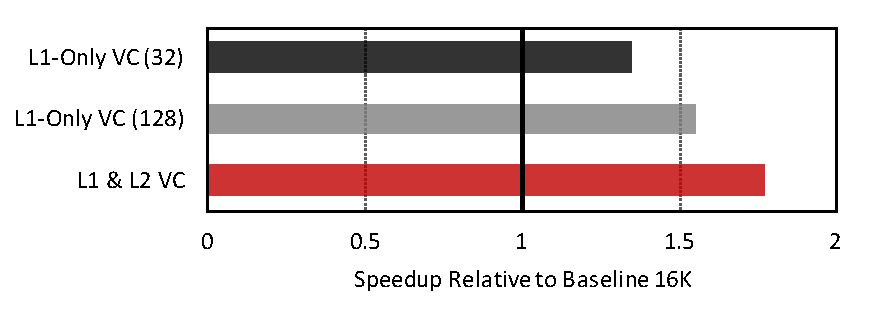
\includegraphics[width=0.95\linewidth]
    {figures/L1VC.pdf}}
  \caption{Proposed GPU virtual cache hierarchy.}
  \label{figure:VCDSR_GPU}
\end{figure}
\subsection{Tolerating introduced latency}
\subsection{Issues with present scheme(not one-to-one and increased tag size)}
Given that the mapping from set number obtained from the set index bits of the original address to the actual set in which the data item is cached is many to many, the original tag bits alone would not suffice to uniquely identify the addresses that get mapped to the particular set. This would entail having to use larger tags in the L1 cache. In effect, because of the many to many mapping from original set number to the mapped set number, our tag size increases to the size of a tag in a fully associative cache. However, the tag comparison is still to be performed only amongst the tags present in the particular set of interest.   <Roughly quote the amount of 



\section{Background and Related Work}
Side channel is an unintentional leakage of information from a victim to an adversary because of the implementation of the hardware and the way of usage \cite{szefer2019survey}. Software guarantees isolation of the data, but the side channels bypass these guarantess and leak data. Cache based side channel attacks leak information about which addresses are referenced and in what order. When secrets are used to index into a data structure, it has the potential to leak information about the secret. This is common in a lot of implementations of cryptographic algorithms, where we have table lookups, for which the index comes from certain bits of the key. Examples of the same are multiplier tables in the RSA algorithm, which is implemented as a lookup table, for which the index comes from bits of the key \cite{liu2014random}.

Cache based side channel attacks can be broadly classified into \textit{conflict based attacks} \cite{deng2019analysis} and \textit{reuse based attacks}.

Conflict based attacks happen when the attacker and victim contend for the same cache set. The attacker exploits the deterministic nature of the mapping from addresses to sets, to learn information about the victim's address. Classic example of this kind of an attack is the Prime and Probe \cite{percival2005cache} \cite{osvik2006cache}. Here, the attacker first primes or fills one or more sets of the cache with his data. Then the attacker waits for the victim to run, and subsequently accesses the items to see if all the items are still cached. If any of the items see a longer access time, then the attacker knows which of his data items got evicted by the victim, and thereby learns information about the set in the cache, that saw contention from the victim. Our work seeks to mitigate these kinds of attacks, where the attack relies on learning the location of a memory line in the cache. 
Prior solutions to mitigate conflict based attacks in the L1 cache such as RPCache \cite{wang2007new} and NewCache \cite{wang2008novel} require large table lookups, and also require making changes to the address decoder logic within the cache to tolerate the additional latency introduced, which our scheme avoids. CEASER \cite{qureshi2018ceaser} uses an encrypted line address to index the cache, whereas application of a similar solution in the L1 cache is expensive, because the L1 cache access is on the critical path. <Given they perform an explicit remap after some time interval, you mention that it affects the quiescient state of the cache, could you help us elaborate> Other approaches such as way partitioning (static or dynamic) that seek to partition the ways of a cache across different protection domains \cite{wang2016secdcp} \cite{liu2016catalyst} \cite{domnitser2012non} \cite{kiriansky2018dawg} lead to under-utilization of cache space and become less feasible in the context of an L1 cache, where space is more of a premium. PLCache \cite{wang2007new} requires locking of certain cache lines, which again leads to under-utilization of cache space.

Reuse Based attacks in contrast do not rely on the location of the memory line in the cache and instead only rely on the fact that a line that was accessed previoiusly will be cached and a subsequent reference would result in a cache hit. These attacks are possible when there is data that is shared between the attacker and the victim. An example of such an attack is the Flush+Reload attack \cite{yarom2014flush+}. Here, the attacker can directly access the target addresses (unlike in the case of conflict based attack, where the attacker was using conflicting addresses to launch the attack), for example if the target addresses are a part of a shared library. The attacker has to run \textit{clflush} \cite{guide2016intel} instruction, to flush all the target addresses from the cache. This gives a guarantee that the addresses have indeed been written back to memory and invalidated in the caches. Then, the attacker lets the victim run, and subsequently measures the time to access each of the target lines he had flushed. If any of the target addresses hit in the cache, it would have a lower access time, giving the attacker information about the address that was accessed.   


\section{Security Analysis}
Talk about our attack model here. 


\section{Evaluation Methodology}


\section{Performance Impact}
There are a few reasons for change in peformance with the changes we introduce. Firstly, we affect the placement of blocks in the cache, which affects the number of cache misses. We have extra logic to compute the new set index from the address bits, for all the three design schemes proposed. This has the potential to introduce additional latency before we can access the L1 cache, and could affect performance. For the last scheme, we have a table containing the hash scheme that has to be looked up, before we can compute the modified index. This again has the potential to add extra latency before we can access the L1 cache.   

\begin{table}[h]
	\caption {Impact of Design on MPKI}
	\begin{tabular}{|c||c||c||c||c||c|}
	      \hline
		Workload Name & Baseline & Single Hash Scheme & Multiple Static Hash Schemes & Changing Hash Schemes & Fully Associative\\
	      \hline
		astar & 35.21 & 20.45 & 18.26 & 16.47 & 5.12\\
	      \hline
		milc & 69.54 & 69.63 & 69.63 & 69.64 & 69.62\\
	      \hline
		soplex & 91.58 & 91.48 & 91.57 & 91.5 & 91.5 \\ 
	      \hline
		sphinx3 & 60.26 & 60.0 & 59.84 & 59.936 & 59.688\\
	      \hline
		zeusmp & 34.75 & 35.20 & 34.97 & 35.26 & 35.281\\
	      \hline
		GemsFDTD & 55.86 & 48.79 & 48.88 & 48.85 & 48.45\\
	      \hline
		lbm & 88.34 & 87.48 & 88.61 & 88.64 & 91.464\\
	      \hline
		bwaves & 0.45 & 0.44 & 0.48 & 0.45 & 0.45\\
	      \hline 
		namd & 12.41 & 11.65 & 17.31 & 16.77 & 7.36\\
	      \hline
		calculix & 32.82 & 33.01 & 33.85 & 33.33 & 33.11\\
	      \hline
		leslie3d & 83.52 & 85.02 & 85.26 & 84.55 & 82.486\\
	      \hline
		gromacs  & 29.18 &29.29 & 29.20 & 29.41 & 29.29\\
	      \hline
		bzip2 & 19.47 & 18.88 & 18.94 & 18.92 & 18.21\\
	      \hline
		mcf & 24.85 & 24.68 & 24.45 & 24.41 & 23.69\\
	      \hline
		hmmer & 0.78 & 0.69 & 0.84 & 0.69 & 0.47\\
	      \hline
		h264ref & 9.69 & 9.64 & 11.16 & 10.365 & 10.248\\
	      \hline
		omnetpp & 19.58 & 19.69 & 19.39 & 19.64 & 20.4795\\
	      \hline 
		sjeng & 7.47 & 8.219 & 7.429 & 6.96 & 6.318\\
	      \hline
		libquantum & 132.11 & 132.11 & 132.10 & 132.11 & 132.11\\
	      \hline
	  \end{tabular}
\end{table}

\subsection {Impact on Cache Misses}
We measure the impact on number of cache misses by measuring the MPKI  for different applications. The MPKI improves a lot for \textit{astar} as well as \textit{GemsFDTD}. This is not unexpected, as was studied by Seznec et.al \cite{seznec1993case}, allowing placement of blocks at different locations in the cache. It has the benefit of adding more associativity and bringing down the number of conflict misses. To validate this assumption of ours, we also run the applications with a fully associative cache, to understand how much benefit the different applications see from bringing down all conflict misses. The same applications, namely \textit{astar} and \textit{GemsFDTD}, see most benefit from moving to a fully associative cache and the other applications are negligibly impacted by increase in associativity, which ties in well with the observations we made with our cache placement strategy.   
\subsection {Storage Overheads} <table storage>
Size of each tag goes up by 9 bits, which is the size of a tag in a fully associative cache. This allows us to reap the performance benefit of reduced conflict misses as well as the security benefit of having a single set and no information leaking from the knowledge about an eviction. For a 64kB cache with 2 ways of associativity, this would be a total of around 576B of extra storage.    
For our third scheme, we have a table that is indexed using the lower bits of the page number. <not sure how to quantify the storage overhead for the table we introduce to lookup the scheme to use, when we have changing schemes> 
\subsection {Impact on Latency} <table lookup latency and hash computation latency>
For the third design, we have a table lookup to figure out the hashing scheme that is to be used. The latency of this table lookup can be hidden by overlapping it with the process of address generation. The contents of the base register can be used to extract the virtual page number, whose lower bits are used to index the table. There could be an overflow when adding the base and offset register, however the access would just go to the next virtual page in this case. One can simply use the scheme corresponding to page number (VPN) obtained from the base register and VPN+1. Then select one of the schemes based on whether there was an overflow or not, when adding the base register with the offset.
For all the three designs, the commonality is that we have to XOR different set of bits from address with each other to obtain the modified set index. This incurs extra latency, <latch logic to tolerate this additional latency> 
\subsection{Sensitivity to associativity}



\section{Conclusions}


\section{Acknowledgements}





%\subsection{Paper Formatting}
%
%Papers must be submitted in printable PDF format and should contain a
%{\bf maximum of 11 pages} of single-spaced two-column text, {\bf not
%  including references}.  You may include any number of pages for
%references, but see below for more instructions.  If you are using
%\LaTeX~\cite{lamport94} to typeset your paper, then we suggest that
%you use the template here:
%\href{http://www.microarch.org/micro50/micro50-latex-template.tar.gz}{\LaTeX~Template}. This
%document was prepared with that template.  If you use a different
%software package to typeset your paper, then please adhere to the
%guidelines given in Table~\ref{table:formatting}.
%
%\begin{scriptsize}
%\begin{table}[h!]
%  \centering
%  \begin{tabular}{|l|l|}
%    \hline
%    \textbf{Field} & \textbf{Value}\\
%    \hline
%    \hline
%    File format & PDF \\
%    \hline
%    Page limit & 11 pages, {\bf not including}\\
%               & {\bf references}\\
%    \hline
%    Paper size & US Letter 8.5in $\times$ 11in\\
%    \hline
%    Top margin & 1in\\
%    \hline
%    Bottom margin & 1in\\
%    \hline
%    Left margin & 0.75in\\
%    \hline
%    Right margin & 0.75in\\
%    \hline
%    Body & 2-column, single-spaced\\
%    \hline
%    Space between columns & 0.25in\\
%    \hline
%    Body font & 10pt, Times\\
%    \hline
%    Abstract font & 10pt, Times, italicized\\
%    \hline
%    Section heading font & 12pt, bold\\
%    \hline
%    Subsection heading font & 10pt, bold\\
%    \hline
%    Caption font & 9pt (minimum), bold\\
%    \hline
%    References & 8pt, no page limit, list \\
%               & all authors' names\\
%    \hline
%  \end{tabular}
%  \caption{Formatting guidelines for submission.}
%  \label{table:formatting}
%\end{table}
%\end{scriptsize}
%
%\textbf{Please ensure that you include page numbers with your
%submission}. This makes it easier for the reviewers to refer to different
%parts of your paper when they provide comments.
%
%Please ensure that your submission has a banner at the top of the
%title page, similar to
%\href{http://www.microarch.org/micro50/samplepaper.pdf}{this one},
%which contains the submission number and the notice of
%confidentiality.  If using the template, just replace XXX with your
%submission number.
%
%\subsection{Content}

%\noindent\textbf{\sout{Author List.}} Reviewing will be double blind;
%therefore, please do not include any author names on any submitted
%documents except in the space provided on the submission form.  You must
%also ensure that the metadata included in the PDF does not give away the
%authors. If you are improving upon your prior work, refer to your prior
%work in the third person and include a full citation for the work in the
bibliography.  For example, if you are building on {\em your own} prior
work in the papers \cite{nicepaper1,nicepaper2,nicepaper3}, you would say
something like: "While the authors of
\cite{nicepaper1,nicepaper2,nicepaper3} did X, Y, and Z, this paper
additionally does W, and is therefore much better."  Do NOT omit or
anonymize references for blind review.  There is one exception to this for
%your own prior work that appeared in IEEE CAL, workshops without archived
%proceedings, etc.\, as discussed later in this document.

%\noindent\textbf{Figures and Tables.} Ensure that the figures and tables
%are legible.  Please also ensure that you refer to your figures in the main
%text.  Many reviewers print the papers in gray-scale. Therefore, if you use
%colors for your figures, ensure that the different colors are highly
%distinguishable in gray-scale.
%
%\noindent\textbf{References.}  There is no length limit for references.
%{\bf Each reference must explicitly list all authors of the paper. Papers
%not meeting this requirement will be rejected.} Authors of NSF proposals
%should be familiar with this requirement. Knowing all authors of related
%work will help find the best reviewers. Since there is no length limit 
%for the number of pages used for references, there is no need to save space 
%here. 


%\subsection{Guidelines for Determining Authorship}
%
%IEEE guidelines dictate that authorship should be based on a {\bf
%substantial intellectual contribution}. It is assumed that all
%authors have had a significant role in the creation of an article that
%bears their names. In particular, the authorship credit must be
%reserved only for individuals who have met each of the following
%conditions:
%
%\begin{enumerate}
%
%\item Made a significant intellectual contribution to the theoretical
%  development, system or experimental design, prototype development,
%  and/or the analysis and interpretation of data associated with the
%  work contained in the article;
%
%\item Contributed to drafting the article or reviewing and/or revising
%  it for intellectual content; and
%
%\item Approved the final version of the article as accepted for
%  publication, including references.
%
%\end{enumerate}
%
%A detailed description of the IEEE authorship guidelines and
%responsibilities is available
%\href{https://www.ieee.org/publications_standards/publications/rights/Section821.html}{here}.
%Per these guidelines, it is not acceptable to award {\em honorary }
%authorship or {\em gift} authorship. Please keep these guidelines in
%mind while determining the author list of your paper.
%
%
%\subsection{Declaring Authors}
%
%Declare all the authors of the paper upfront. Addition/removal of authors
%once the paper is accepted will have to be approved by the program chairs,
%since it potentially undermines the goal of eliminating conflicts for
%reviewer assignment.
%
%
%\subsection{Areas and Topics}
%
%Authors should indicate these areas on the submission form as
%well as specific topics covered by the paper for optimal reviewer match. If
%you are unsure whether your paper falls within the scope of MICRO, please
%check with the program chairs---MICRO is a broad, multidisciplinary
%conference and encourages new topics.
%
%\subsection{Declaring Conflicts of Interest}
%
%Authors must register all their conflicts on the paper submission site.
%Conflicts are needed to ensure appropriate assignment of reviewers.  
%If a paper is found to have an undeclared conflict that causes
%a problem OR if a paper is found to declare false conflicts in order to
%abuse or ``game'' the review system, the paper may be rejected.
%
%We use the NSF conflict of interest guidelines for determining the
%conflict period for MICRO 2017.  Please declare a conflict of interest
%(COI) with the following people for any author of your paper:
%
%\begin{enumerate}
%\item Your Ph.D. advisor(s), post-doctoral advisor(s), Ph.D. students, 
%      and post-doctoral advisees, forever. 
%\item Family relations by blood or marriage, or their equivalent, 
%      forever (if they might be potential reviewers).
%\item People with whom you have collaborated in the last FOUR years, including 
%\begin{itemize}
%\item co-authors of accepted/rejected/pending papers.
%\item co-PIs on accepted/rejected/pending grant proposals.
%\item funders (decision-makers) of your research grants, and researchers 
%      whom you fund. 
%\end{itemize}
%\item People (including students) who shared your primary institution(s) in the 
%last FOUR years. 
%\item Other relationships, such as close personal friendship, that you think might tend
%to affect your judgment or be seen as doing so by a reasonable person familiar
%with the relationship.
%\end{enumerate}
%
%``Service'' collaborations such as co-authoring a report for a professional 
%organization, serving on a program committee, or co-presenting 
%tutorials, do not themselves create a conflict of interest. 
%Co-authoring a paper that is a compendium of various projects with 
%no true collaboration among the projects does not constitute a 
%conflict among the authors of the different projects.
%
%On the other hand, there may be others not covered by the above with
%whom you believe a COI exists, for example, an ongoing collaboration
%which has not yet resulted in the creation of a paper or proposal.
%Please report such COIs; however, you may be asked to justify them.
%Please be reasonable. For example, you cannot declare a COI with a
%reviewer just because that reviewer works on topics similar to or
%related to those in your paper.  The PC Chair may contact co-authors
%to explain a COI whose origin is unclear.
%
%We hope to draw most reviewers from the PC and the ERC, but others from the
%community may also write reviews.  Please declare all your conflicts (not
%just restricted to the PC and ERC).  When in doubt, contact the program
%chairs.
%
%
%\subsection{Concurrent Submissions and Workshops}
%
%By submitting a manuscript to MICRO 2017, the authors guarantee that the
%manuscript has not been previously published or accepted for publication in
%a substantially similar form in any conference, journal, or the archived
%proceedings of a workshop (e.g., in the ACM digital library) -- see
%exceptions below. The authors also guarantee that no paper that contains
%significant overlap with the contributions of the submitted paper will be
%under review for any other conference or journal or an archived proceedings
%of a workshop during the MICRO 2017 review period. Violation of any of these
%conditions will lead to rejection.
%
%The only exceptions to the above rules are for the authors' own papers
%in (1) workshops without archived proceedings such as in the ACM
%digital library (or where the authors chose not to have their paper
%appear in the archived proceedings), or (2) venues such as IEEE CAL
%where there is an explicit policy that such publication does not
%preclude longer conference submissions.  In all such cases, the
%submitted manuscript may ignore the above work to preserve author
%anonymity. This information must, however, be provided on the
%submission form---the PC chairs will make this information available
%to reviewers if it becomes necessary to ensure a fair review.  As
%always, if you are in doubt, it is best to contact the program chairs.
%
%
%Finally, the ACM Plagiarism Policy ({\em
%http://www.acm.org/publications/policies/plagiarism\_policy}) covers a
%range of ethical issues concerning the misrepresentation of other works or
%one's own work.



%%%%%%% -- PAPER CONTENT ENDS -- %%%%%%%%


%%%%%%%%% -- BIB STYLE AND FILE -- %%%%%%%%
\bibliographystyle{IEEEtranS}
\bibliography{refs}
%%%%%%%%%%%%%%%%%%%%%%%%%%%%%%%%%%%%

\end{document}
